
\textbf{2019.10.14}

Állapotok:
\begin{itemize}
\item READY
	\begin{itemize}
	\item Alap állapot 
	\item "reset" jel esetén ide kerül vissza az automata
	\end{itemize}
\item INIT
	\begin{itemize}
	\item minden LED-et kikapcsol (0x000000-t ír)
	\item "clear" jel esetén ide kerül az automata
	\end{itemize}
\item RENDER
	\begin{itemize}
	\item egyenként küldi a szín információt a LED-ekre
	\item annyiszor végződik el itt a művelet, ahány LED-ünk van
	\item "stop" jel esetén megáll a kiírás
	\end{itemize}
\item DISPLAY
	\item megtörtént a kiírás
\end{itemize}

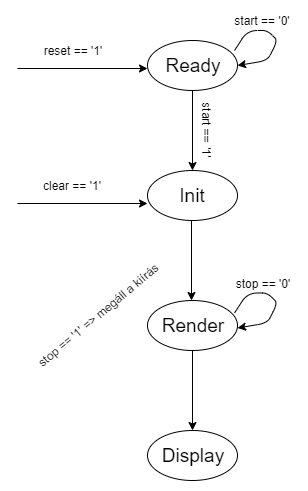
\includegraphics[scale=0.5]{allapotdiagram.png}

\textbf{2019.10.28}

Állapotdiagram átírva úgy, hogy a küldési logikát is tartalmazza:

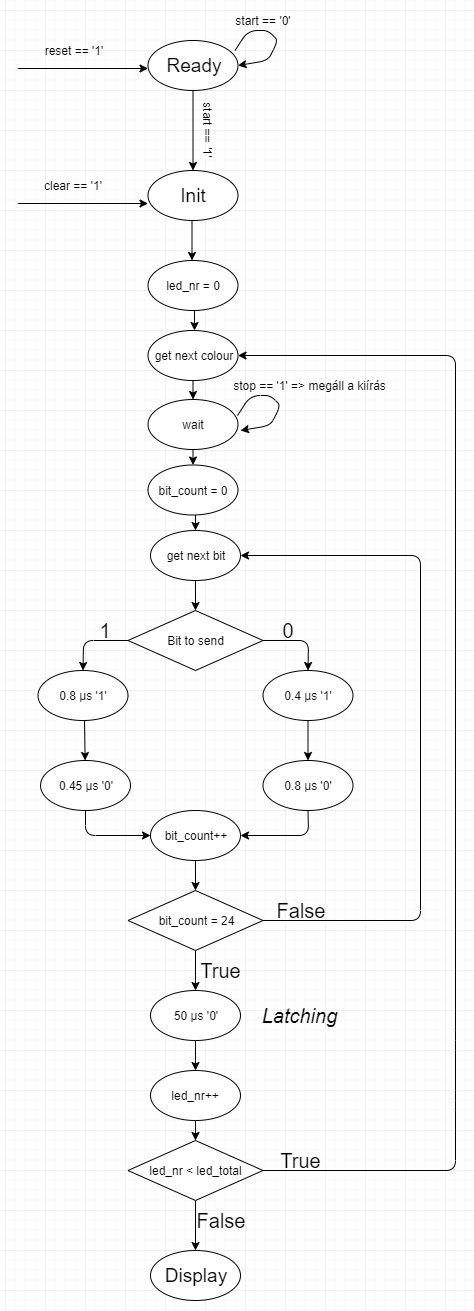
\includegraphics[scale=0.4]{allapotdiagram_2.png}

Állapotdiagram egy 100 LED-et vezérlő modulra

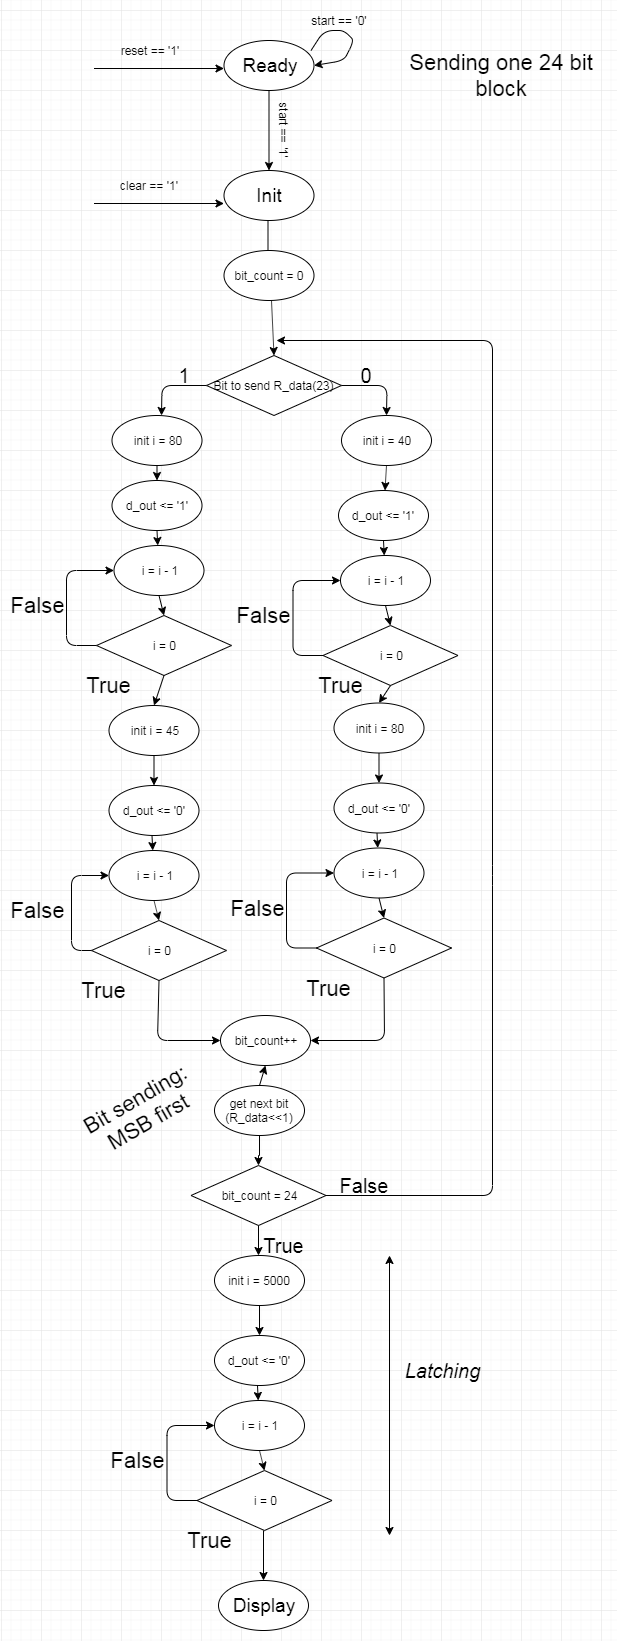
\includegraphics[scale=0.4]{allapotdiagram_3.png}

\textbf{2019.11.11}

Végleges állapotdiagram, az implementációban is használt.

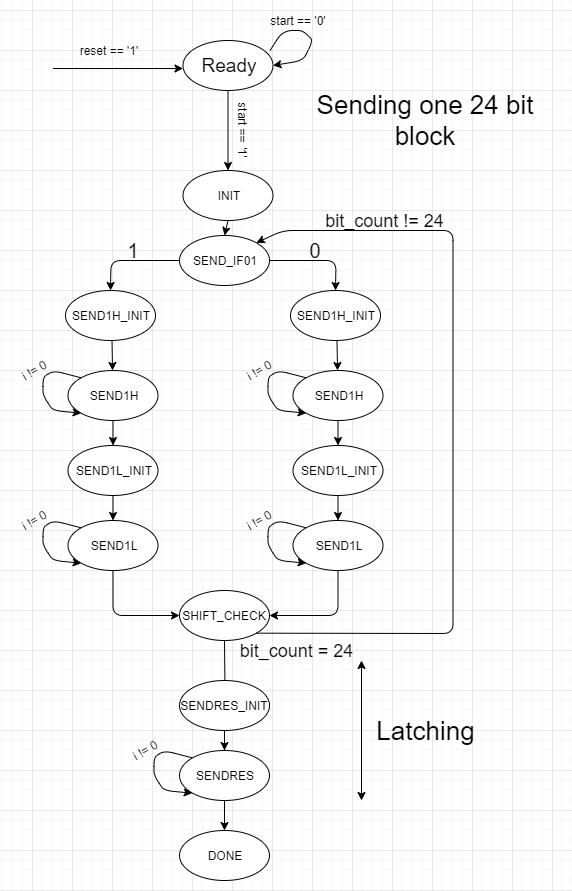
\includegraphics[scale=0.5]{allapotdiagram_final.png}

\begin{itemize}
\item READY
	\begin{itemize}
	\item Alap állapot 
	\item "reset" jel esetén ide kerül vissza az automata
	\end{itemize}
\item INIT
	\begin{itemize}
	\item inicializálja a bit-count-ot nullára
	\end{itemize}
\item SENDIF\_01
	\begin{itemize}
	\item Megvizsgálja data[23]-as bit-et. Ha 1, akkor a következő állapot a \textbf{SEND1H\_INIT}, ha 0 akkor SEND0H\_INIT
	\end{itemize}
\item SEND1H\_INIT
	\begin{itemize}
	\item Inicializálja az \textbf{i} változót a T1H értékre
	\item A d\_out output-ot 1-re állítja
	\end{itemize}
\item SEND1H
	\begin{itemize}
	\item Dekrementálja az \textbf{i} változót
	\item Amikor az \textbf{i} változó nulla lesz, akkor tovább megy a \textbf{SEND1L\_INIT} állapotra
	\end{itemize}
\item SEND1L\_INIT
	\begin{itemize}
	\item Inicializálja az \textbf{i} változót a T1L értékre
	\item A d\_out output-ot 0-ra állítja
	\end{itemize}
\item SEND1L
	\begin{itemize}
	\item Dekrementálja az \textbf{i} változót
	\item Amikor az \textbf{i} változó nulla lesz, akkor tovább megy a \textbf{SHIFT\_CHECK} állapotra
	\end{itemize}
\item SEND0H\_INIT
	\begin{itemize}
	\item Inicializálja az \textbf{i} változót a T0H értékre
	\item A d\_out output-ot 1-re állítja
	\end{itemize}
\item SEND0H
	\begin{itemize}
	\item Dekrementálja az \textbf{i} változót
	\item Amikor az \textbf{i} változó nulla lesz, akkor tovább megy a \textbf{SEND0L\_INIT} állapotra
	\end{itemize}
\item SEND0L\_INIT
	\begin{itemize}
	\item Inicializálja az \textbf{i} változót a T0L értékre
	\item A d\_out output-ot 0-ra állítja
	\end{itemize}
\item SEND0L
	\begin{itemize}
	\item Dekrementálja az \textbf{i} változót
	\item Amikor az \textbf{i} változó nulla lesz, akkor tovább megy a \textbf{SHIFT\_CHECK} állapotra
	\end{itemize}
\item SHIFT\_CHECK
	\begin{itemize}
	\item Megnézi, hogy a \textbf{bit\_count} változó nulla-e, ha igen, akkor tovább megy a \textbf{SENDRES\_INIT} állapotra
	\item Ha a \textbf{bit\_count} változó nem egyenlő nullával, akkor tovább megy a \textbf{SHIFT} állapotra
	\end{itemize}
\item SHIFT
	\begin{itemize}
	\item Shift-eli a \textbf{data} std logic vectort balra eggyel; vissza megy a \textbf{SEND\_IF01} állapotra
	\end{itemize}
\item SENDRES\_INIT
	\begin{itemize}
	\item Inicializálja az \textbf{i} változót a TRES értékre
	\item A d\_out output-ot 0-ra állítja
	\end{itemize}
\item SENDRES
	\begin{itemize}
	\item Dekrementálja az \textbf{i} változót
	\item Amikor az \textbf{i} változó nulla lesz, akkor tovább megy a \textbf{SEND\_DONE} állapotra
	\end{itemize}
\item SEND\_DONE
	\begin{itemize}
	\item Befejeződött a 24 bit-es blokk kiírása
	\item Beállítja a \textbf{done} kimenetet 1-esre
	\end{itemize}
\end{itemize}